\newpage
\section{Ôn tập chương 9}
\def\thoigian{90}%--Thời gian
\de{Đề số 1}{Chương IX. Xác suất}

\begin{center}
	\textbf{PHẦN 1 - CÂU TRẮC NGHIỆM BỐN PHƯƠNG ÁN}
\end{center}
\Opensolutionfile{ans}[ans/1T9-OTC-Deso1-TN]

%Câu 1
\begin{ex}%[1D9N2-1]%[Dự án D đợt 3 - Đề ôn tập chương Xác Suất]%[Ngô Tất Thành]
	Hai biến cố $A$ và $B$ được gọi là xung khắc khi và chỉ khi
	\choice
	{$A \cup B=\Omega$}
	{$A \cup B=\varnothing$}
	{$A \cap B=\Omega$}
	{\True $A \cap B=\varnothing$}
	\loigiai{
		Hai biến cố $A$ và $B$ được gọi là xung khắc khi và chỉ khi $A \cap B=\varnothing$.}
\end{ex}

%Câu 2
\begin{ex}%[1D9H1-2]%[Dự án D đợt 3 - Đề ôn tập chương Xác Suất]%[Ngô Tất Thành]
	Một hộp có $5$ quả cầu xanh khác nhau và $6$ quả cầu trắng khác nhau. Lấy ngẫu nhiên đồng thời $2$ quả cầu. Có bao nhiêu cách lấy ra hai quả cầu cùng màu? 
	\choice
	{$10$}
	{$15$}
	{\True $25$}
	{$55$}
	\loigiai{
		Gọi biến cố $A$: \lq\lq Lấy ra hai quả cầu màu xanh\rq\rq.\\
		Biến cố $B$: \lq\lq Lấy ra hai quả cầu màu trắng\rq\rq.\\
		Biến cố $H$: \lq\lq Lấy ra hai quả cầu cùng màu\rq\rq.\\
		Khi đó $H=A\cup B$ và $A\cap B=\varnothing$.\\
		Do hai biến cố $A$ và $B$ là xung khắc nên $n(H)=n(A)+n(B)$\\
		Số các kết quả thuận lợi cho biến cố $A$ là $n(A)=\mathrm{C}_5^2=10$.\\
		Số các kết quả thuận lợi cho biến cố $B$ là $n(B)=\mathrm{C}_6^2=15$.\\
		Số các kết quả thuận lợi cho biến cố $H$ là $n(H)=n(A)+n(B)=10+15=25$.
	}
\end{ex}

%Câu 3
\begin{ex}%[1D9N1-1]%[Dự án D đợt 3 - Đề ôn tập chương Xác Suất]%[Ngô Tất Thành]
	Gieo ngẫu nhiên một con xúc sắc cân đối và đồng chất hai lần liên tiếp. $A$ là biến cố \lq\lq Số chấm xuất hiện ở lần thứ nhất là số lẻ\rq\rq, $B$ là biến cố \lq\lq Số chấm xuất hiện ở lần thứ hai là số lẻ\rq\rq. Chọn khẳng định đúng.
	\choice
	{Hai biến cố $A$ và $B$ xung khắc}
	{$A$ và $B$ là hai biến cố đối nhau}
	{Biến cố giao của hai biến cố $A$ và $B$ là \lq\lq Số chấm xuất hiện ở lần thứ nhất hoặc lần thứ hai là số lẻ\rq\rq}
	{\True Biến cố giao của hai biến cố $A$ và $B$ là \lq\lq Số chấm xuất hiện hai lần gieo đều là số lẻ\rq\rq}
	\loigiai{
		$A \cap B$ là \lq\lq Số chấm xuất hiện ở lần thứ nhất là số lẻ và số chấm xuất hiện ở lần thứ hai là số lẻ\rq\rq.
	}
\end{ex}

%Câu 4
\begin{ex}%[1D9H1-3]%[Dự án D đợt 3 - Đề ôn tập chương Xác Suất]%[Ngô Tất Thành]
	Cho $A$, $B$ là hai biến độc lập với nhau, biết $\mathrm{P}(A)=0{,}4$; $\mathrm{P}(B)=0{,}3$. Khi đó $\mathrm{P}(AB)$ bằng
	\choice
	{$0{,}1$}
	{\True $0{,}12$}
	{$0{,}58$}
	{$0{,}7$} 
	\loigiai{
		Ta có $\mathrm{P}(AB)=\mathrm{P}(A) \cdot \mathrm{P}(B)=0{,}4\cdot 0{,}3=0{,}12$.
	}
\end{ex}

%Câu 5
\begin{ex}%[1D9H1-1]%[Dự án D đợt 3 - Đề ôn tập chương Xác Suất]%[Ngô Tất Thành]
	Cho $A$ và $B$ là hai biến cố. Biết $\mathrm{P}(\overline{A})=0{,}7$; $\mathrm{P}(B)=0{,}3$; $\mathrm{P}(AB)=0{,}21$. Mệnh đề nào đúng?
	\choice
	{$A$ và $B$ là hai biến cố xung khắc}
	{$A$ và $B$ là hai biến cố đối}
	{$A$ và $B$ là hai biến cố độc lập}
	{\True $A$ và $B$ là hai biến cố không độc lập}
	\loigiai{
		Ta có $\mathrm{P}(A)=1-0{,}7=0{,}3$.\\
		Do $\mathrm{P}(A) \cdot \mathrm{P}(B)=0{,}3\cdot 0{,}3=0{,}09\neq \mathrm{P}(AB)$ nên hai biến cố $A$ và $B$ không độc lập.
	}
\end{ex}

%Câu 6
\begin{ex}%[1D9H1-3]%[Dự án D đợt 3 - Đề ôn tập chương Xác Suất]%[Ngô Tất Thành]
	Có ba vận động viên cùng thi chạy vượt rào. Xác suất để ba vận động viên này vượt qua được rào lần lượt là $0{,}9$; $0{,}8$; $0{,}7$. Tìm xác suất để cả ba vận động viên vượt qua được rào.
	\choice
	{$\mathrm{P}=0{,}398$}
	{$\mathrm{P}=0{,}994$}
	{\True $\mathrm{P}=0{,}504$}
	{$\mathrm{P}=0{,}72$}
	\loigiai{
		Gọi biến cố $A$: \lq\lq Cả ba vận động viên vượt qua được rào\rq\rq.\\
		$A_i$: \lq\lq Vận động viên thứ $i$ vượt qua được rào\rq\rq\, với $i \in\{1; 2; 3\}$.\\
		Vậy $\mathrm{P}(A)=\mathrm{P}\left(A_1\right) \cdot \mathrm{P}\left(A_2\right) \cdot \mathrm{P}\left(A_3\right)=0{,}9\cdot 0{,}8\cdot 0{,}7=0{,}504$.
	}
\end{ex}

%Câu 7
\begin{ex}%[1D9H2-4]%[Dự án D đợt 3 - Đề ôn tập chương Xác Suất]%[Ngô Tất Thành]
	Cho $A$ và $B$ là hai biến cố độc lập. Biết $\mathrm{P}(A) = 0{,}5$ và $\mathrm{P}(A \cap B) = 0{,}2$. Xác suất $\mathrm{P}(A\cup B)$ bằng
	\choice
	{$0{,}3$}
	{$0{,}5$}
	{$0{,}6$}
	{\True $0{,}7$}
	\loigiai{
		Vì $A$ và $B$ là hai biến cố độc lập nên
		\[\mathrm{P}(A \cap B) = \mathrm{P}(A) \cdot \mathrm{P}(B) \Rightarrow \mathrm{P}(B) = \dfrac{\mathrm{P}(A \cap B)}{\mathrm{P}(A)} = \dfrac{0{,}2}{0{,}5} = 0{,}4.\]
		Do đó
		\[\mathrm{P}(A \cup B) = \mathrm{P}(A) + \mathrm{P}(B) - \mathrm{P}(A \cap B) = 0{,}5 + 0{,}4 - 0{,}2 = 0{,}7.\]
	}
\end{ex}


%Câu 8
\begin{ex}%[1D9H2-3]%[Dự án D đợt 3 - Đề ôn tập chương Xác Suất]%[Ngô Tất Thành]
	Một hộp đựng $5$ quả cầu màu xanh và $3$ quả cầu màu đỏ có cùng kích thước và khối lượng. Chọn ngẫu nhiên hai quả cầu trong hộp. Tính xác suất để chọn được hai quả cầu có cùng màu.
	\choice
	{$\dfrac{10}{28}$}
	{$\dfrac{3}{28}$}
	{\True $\dfrac{13}{28}$}
	{$\dfrac{1}{2}$}
	\loigiai{Xét các biến cố
		\begin{itemize}
			\item $A$: \lq \lq Chọn được cả hai quả cầu màu xanh\rq\rq.
			\item $B$: \lq \lq Chọn được cả hai quả cầu màu đỏ\rq \rq. 
		\end{itemize} 
		Biến cố  $C$: \lq \lq Hai quả cầu có cùng màu\rq \rq \ là biến cố hợp của $A$ và $B$. \\
		Hai biến cố $A$ và $B$ là xung khắc nên $\mathrm{P}(C) = \mathrm{P}(A) + \mathrm{P}(B)$.\\
		Ta có
		\[n(\Omega) = \mathrm{C}_8^2 = 28, \ n(A) = \mathrm{C}_5^2 = 10, \ n(B) = \mathrm{C}_3^2 = 3.\]
		Do đó
		\[\mathrm{P}(A) = \dfrac{10}{28}, \ \mathrm{P}(B) = \dfrac{3}{28}.\]
		Vậy
		\[\mathrm{P}(C) = \mathrm{P}(A) + \mathrm{P}(B) = \dfrac{10}{28} + \dfrac{3}{28} = \dfrac{13}{28}.\]
	}
\end{ex}

%Câu 9
\begin{ex}%[1D9H2-3]%[Dự án D đợt 3 - Đề ôn tập chương Xác Suất]%[Ngô Tất Thành]
	Một chiếc hộp có $10$ chiếc thẻ cùng loại được đánh số từ $1$ đến $10$. Rút ngẫu nhiên từ hộp ra $1$ thẻ. Xét các biến cố
	\begin{enumerate}
		\item[$A$:] \lq\lq Số ghi trên thẻ được lấy ra là số lớn hơn $6$\rq \rq.  
		\item[$B$:] \lq \lq Số ghi trên thẻ được lấy ra là không vượt quá $5$\rq \rq.
	\end{enumerate}
	Tính xác suất của biến cố $A \cup B$?
	\choice
	{$0{,}4$}
	{\True $0{,}9$}
	{$0{,}5$}
	{$0{,}36$}
	\loigiai{
		Không gian mẫu có $n(\Omega) = 10$.\\
		Biến cố $A$: \lq \lq Số ghi trên thẻ được lấy ra là số lớn hơn $6$\rq \rq.
		\[A = \{7; 8; 9; 10\} \Rightarrow n(A) = 4.\] 
		\[\mathrm{P}(A) = \dfrac{n(A)}{n(\Omega)} = \dfrac{4}{10} = 0{,}4.\]
		Biến cố $B$: \lq\lq Số ghi trên thẻ được lấy ra là không vượt quá $5$\rq \rq.
		\[B = \{1; 2; 3; 4; 5\} \Rightarrow n(B) = 5.\]
		\[\mathrm{P}(B) = \dfrac{n(B)}{n(\Omega)} = \dfrac{5}{10} = 0{,}5.\]
		Vì $A$, $B$ là hai biến cố xung khắc nên
		\[\mathrm{P}(A \cup B) = \mathrm{P}(A) + \mathrm{P}(B) = 0{,}4 + 0{,}5 = 0{,}9.\]
	}
\end{ex}

%Câu 10
\begin{ex}%[1D9H2-3]%[Dự án D đợt 3 - Đề ôn tập chương Xác Suất]%[Ngô Tất Thành]
	Một lớp học có $40$ học sinh, gồm $15$ học sinh nam giỏi Toán và $8$ học sinh nữ giỏi Văn. Chọn ngẫu nhiên một học sinh. Tính xác suất để chọn được một nam sinh giỏi Toán hoặc một nữ sinh giỏi Văn.
	\choice
	{$\dfrac{7}{40}$}
	{$\dfrac{1}{5}$}
	{$\dfrac{3}{8}$}
	{\True $\dfrac{23}{40}$}
	\loigiai{
		Gọi $A$ là biến cố: \lq \lq Chọn một nam sinh giỏi Toán\rq \rq.\\  
		Gọi $B$ là biến cố: \lq \lq Chọn một nữ sinh giỏi Văn\rq \rq.  \\
		Khi đó, $A \cup B$ là biến cố \lq \lq Chọn được một nam sinh giỏi Toán hoặc một nữ sinh giỏi Văn\rq \rq. \\ 
		Vì $A$ và $B$ là hai biến cố xung khắc nên $\mathrm{P}(A \cup B) = \mathrm{P}(A) + \mathrm{P}(B)$.\\
		Số phần tử của không gian mẫu là $n(\Omega) = 40$.\\
		Số phần tử của biến cố $A$ và $B$ lần lượt là $n(A) = 15$, $n(B) = 8$. \\
		Xác suất của từng biến cố là
		\[\mathrm{P}(A) = \dfrac{n(A)}{n(\Omega)} = \dfrac{15}{40} = \dfrac{3}{8}, \quad \mathrm{P}(B) = \dfrac{n(B)}{n(\Omega)} = \dfrac{8}{40} = \dfrac{1}{5}.\]
		Vậy xác suất cần tính là
		\[\mathrm{P}(A \cup B) = \mathrm{P}(A) + \mathrm{P}(B) = \dfrac{3}{8} + \dfrac{1}{5} = \dfrac{23}{40}.\]
	}
\end{ex}

%Câu 11
\begin{ex}%[1D9H1-3]%[Dự án D đợt 3 - Đề ôn tập chương Xác Suất]%[Ngô Tất Thành]
	Trong một kỳ thi có $60\%$ thí sinh đỗ. Hai bạn $A$, $B$ cùng dự kỳ thi đó. Xác suất để chỉ có một bạn thi đỗ là
	\choice
	{$0{,}24$}
	{$0{,}36$}
	{$0{,}16$}
	{\True $0{,}48$}
	\loigiai{
		Gọi $A$ là biến cố bạn $A$ thi đỗ, $B$ là biến cố bạn $B$ thi đỗ.\\
		Ta có $\mathrm{P}(A) = \mathrm{P}(B) = 0{,}6 \Rightarrow \mathrm{P}(\overline{A}) = \mathrm{P}(\overline{B}) = 0{,}4$.\\
		Xác suất để chỉ có một bạn thi đỗ là
		\[\mathrm{P} = \mathrm{P}(\overline{A}) \cdot \mathrm{P}(B) + \mathrm{P}(A) \cdot \mathrm{P}(\overline{B}) = 0{,}4 \cdot 0{,}6 + 0{,}6 \cdot 0{,}4 = 0{,}48.\]
	}
\end{ex}

%Câu 12
\begin{ex}%[1D9H2-3]%[Dự án D đợt 3 - Đề ôn tập chương Xác Suất]%[Ngô Tất Thành]
	Có $6$ học sinh gồm $3$ nam và $3$ nữ xếp thành hàng ngang để chụp ảnh. Tính xác suất để các bạn nữ đứng cạnh nhau hoặc nam nữ đứng xen kẽ.  
	\choice
	{\True $\dfrac{3}{10}$}
	{$\dfrac{2}{5}$}
	{$\dfrac{1}{2}$}
	{$\dfrac{1}{50}$}
	\loigiai{
		Không gian mẫu có $n(\Omega) = 6! = 720$.\\
		Gọi biến cố $A$: \lq \lq Ba bạn nữ đứng cạnh nhau\rq \rq.\\
		Khi đó, xem nhóm ba bạn nữ như một đơn vị, cùng với ba bạn nam tạo thành bốn đơn vị cần xếp hàng.  \\
		Số cách sắp xếp các đơn vị này là $	n(A) = 4! \cdot 3! = 144$.\\
		Suy ra $\mathrm{P}(A) = \dfrac{n(A)}{n(\Omega)} = \dfrac{144}{720} = \dfrac{1}{5}$.\\
		Gọi biến cố $B$: \lq \lq Nam nữ đứng xen kẽ\rq\rq. \\
		Khi đó, có hai cách chọn giới tính đứng đầu hàng. Mỗi giới tính có $3!$ cách sắp xếp, nên
		\[n(B) = 2 \cdot 3! \cdot 3! = 72.\]
		Suy ra
		\[	\mathrm{P}(B) = \dfrac{n(B)}{n(\Omega)} = \dfrac{72}{720} = \dfrac{1}{10}.\]
		Do $A, B$ là hai biến cố xung khắc nên
		\[\mathrm{P}(A \cup B) = \mathrm{P}(A) + \mathrm{P}(B) = \dfrac{1}{5} + \dfrac{1}{10} = \dfrac{3}{10}.\]
	}
\end{ex}
\Closesolutionfile{ans}
%\begin{center}
%	\textbf{ĐÁP ÁN}
%	\inputansbox{10}{ans/ans}	
%\end{center}

\begin{center}
	\textbf{PHẦN 2 - CÂU TRẮC NGHIỆM ĐÚNG SAI}
\end{center}
\setcounter{ex}{0}
\Opensolutionfile{ans}[ans/1T9-OTC-Deso1-DS]

%Câu 1
\begin{ex}%[1D9V1-3]%[Dự án D đợt 3 - Đề ôn tập chương Xác Suất]%[Ngô Tất Thành]
	Một xạ thủ bắn lần lượt hai viên đạn vào bia. Xác suất bắn không trúng đích của viên thứ nhất và viên thứ hai lần lượt là $0{,}2$ và $0{,}3$. Gọi biến cố $A$: \lq\lq Lần thứ nhất bắn không trúng bia\rq\rq, biến cố $B$: \lq\lq Lần thứ $2$ bắn không trúng bia\rq\rq.
	\choiceTF
	{\True $A$, $B$ là hai biến cố độc lập}
	{\True Xác suất biến cố: \lq\lq Cả hai lần bắn không trúng bia\rq\rq~là $0{,}06$}
	{\True Xác suất biến cố: \lq\lq Có ít nhất một lần bắn trúng bia\rq\rq~là $0{,}94$}
	{Xác suất biến cố: \lq\lq Lần bắn thứ nhất trúng bia, lần bắn thứ hai không trúng bia\rq\rq~là $0{,}21$}
	\loigiai{
		Ta có $\mathrm{P}(A)=0{,}2$; $\mathrm{P}(B)=0{,}3$; $\mathrm{P}\left(\overline{A}\right)=0{,}8$; $\mathrm{P}\left(\overline{B}\right)=0{,}7$.
		\begin{itemchoice}
			\itemch Vì các kết quả bắn là độc lập với nhau nên $A$, $B$ là hai biến cố độc lập.
			\itemch Biến cố: \lq\lq Cả hai lần bắn đều không trúng bia\rq\rq.\\
			Ta có $A$, $B$ là hai biến cố độc lập nên $\mathrm{P}(AB)=\mathrm{P}(A)\cdot \mathrm{P}(B)=0{,}2\cdot 0{,}3=0{,}06$.
			\itemch Gọi biến cố $D$: “Có ít nhất một lần bắn trúng bia\rq\rq.\\
			Khi đó, biến cố $\overline{D}$: \lq\lq Cả hai lần bắn đều không trúng bia\rq\rq.\\
			Do đó, $\overline{D}=AB$ $\Rightarrow$ $\mathrm{P}\left(\overline{D}\right)=0{,}06$ $\Rightarrow$ $\mathrm{P}(D)=1-\mathrm{P}\left(\overline{D}\right)=0{,}94$.

			\itemch Gọi $C$ là biến cố: \lq\lq Lần bắn thứ nhất trúng bia, lần bắn thứ hai không trúng bia\rq\rq.\\
			Ta có $C=\overline{A}B$ và $\overline{A}$, $B$ là hai biến cố độc lập.\\
			Do đó, $\mathrm{P}(C)=\mathrm{P}\left(\overline{A}\right)\cdot \mathrm{P}(B)=0{,}8\cdot 0{,}3=0{,}24$.
		\end{itemchoice}
	}
\end{ex}

%Câu 2
\begin{ex}%[1D9H2-1]%[Dự án D đợt 3 - Đề ôn tập chương Xác Suất]%[Ngô Tất Thành]
	Một hộp đựng $20$ tấm thẻ cùng loại được đánh số từ $1$ đến $20$. Rút ngẫu nhiên một tấm thẻ trong hộp. Gọi $A$ là biến cố \lq\lq Rút được tấm thẻ ghi số chẵn lớn hơn $9$\rq\rq; $B$ là biến cố \lq\lq Rút được tấm thẻ ghi số từ $9$ đến $14$\rq\rq.
	\choiceTF
	{\True $\mathrm{P}(A)=\dfrac{3}{10}$}
	{\True $\mathrm{P}(A\cup B)=\dfrac{9}{20}$}
	{$A, B$ là hai biến cố xung khắc}
	{$\mathrm{P}(AB)=\dfrac{1}{5}$}
	\loigiai{
		Ta có $A=\{10,12,14,16,18,20\}\Rightarrow n(A)=6$.\\ $B=\{9,10,11,12,13,14\}\Rightarrow n(B)=6$.\\
		$n(\Omega)=20$.
		\begin{itemchoice}
			\itemch $\mathrm{P}(A)=\dfrac{n(A)}{n(\Omega)}=\dfrac{3}{10}$.
			\itemch Ta có $A\cup B=\{9,10,11,12,13,14,16,18,20\}\Rightarrow n(A\cup B)=9$.\\
			Do đó $\mathrm{P}(A\cup B)=\dfrac{n(A\cup B)}{n(\Omega)}=\dfrac{9}{20}$.
			\itemch Hai biến cố $A$ và $B$ không xung khắc vì $A\cap B=\{10,12,14\}$.
			\itemch Ta có $AB=A\cap B=\{10,12,14\}\Rightarrow n(AB)=3$.\\
			Do đó $\mathrm{P}(AB)=\dfrac{n(AB)}{n(\Omega)}=\dfrac{3}{20}$.

		\end{itemchoice}
	}
\end{ex}
\Closesolutionfile{ans}


\begin{center}
\textbf{PHẦN 3 - CÂU TRẮC NGHIỆM TRẢ LỜI NGẮN}
\end{center}
\setcounter{ex}{0}
\Opensolutionfile{ans}[ans/1T9-OTC-Deso1-TLN]

%Câu 1
\begin{ex}%[1D9H1-3]%[Dự án D đợt 3 - Đề ôn tập chương Xác Suất]%[Ngô Tất Thành]
	Trong cuộc thi tranh biện giữa các trường THPT trong thành phố có hai đội là Ngôi Sao và Hoa Mai thuộc hai bảng khác nhau. Mỗi bảng sẽ có một đội có điểm cao nhất vào vòng chung kết. Xác suất để hai đội Ngôi Sao và Hoa Mai đạt được điểm cao nhất lần lượt là $0{,}7$ và $0{,}82$. Tính xác suất để chỉ có đội Ngôi Sao vào chung kết. (Kết quả làm tròn đến hàng phần trăm).
	\shortans{0{,}13}
	\loigiai{
		Gọi $A$ là biến cố: \lq\lq Đội Ngôi Sao được vào chung kết\rq\rq.\\
		$B$ là biến cố: \lq\lq Đội Hoa Mai được vào chung kết\rq\rq.\\
		Theo đề ta có $\mathrm{P}(A)=0{,}7$; $\mathrm{P}(B)=0{,}82$.\\
		Gọi $C$ là biến cố: \lq\lq Chỉ có đội Ngôi Sao được vào chung kết\rq\rq.	\\
		Khi đó $C=A\cap \overline{B}$.\\
		$\mathrm{P}(C)=0{,}7\cdot (1-0{,}82)=0{,}126 \approx 0{,}13$.
	}
\end{ex}

%Câu 2
\begin{ex}%[1D9V1-3]%[Dự án D đợt 3 - Đề ôn tập chương Xác Suất]%[Ngô Tất Thành]
	Một nhà máy có hai tổ máy sản xuất một mặt hàng, biết rằng xác suất để hai tổ máy phải nghỉ để bảo dưỡng lần lượt là $0{,}2$ và $0{,}35$. Tính xác suất để cả hai tổ máy đều hoạt động. 
	\shortans{0{,}52}
	\loigiai{
		Gọi $A$, $B$ lần lượt là biến cố để hai tổ máy nghỉ bảo dưỡng.\\
		Ta có $\mathrm{P}(A)=0{,}2$ và $\mathrm{P}(B)=0{,}35$.\\
		Nên xác suất để hai tổ máy đều hoạt động là $\mathrm{P}\left(\overline{A}\right)=0{,}8$ và $\mathrm{P}\left(\overline{B}\right)=0{,}65$.\\
		Vậy xác suất để cả hai tổ máy đều hoạt động là $\mathrm{P}\left(\overline{A}\cap \overline{B}\right)=0{,}8\cdot 0{,}65=0{,}52$.
	}
\end{ex}


%Câu 3
\begin{ex}%[1D9H2-5]%[Dự án D đợt 3 - Đề ôn tập chương Xác Suất]%[Ngô Tất Thành]
	Tại một trường trung học phổ thông $X$, có $12\%$ học sinh học giỏi môn Tiếng Anh, $35\%$ học sinh học giỏi môn Toán và $8\%$ học sinh học giỏi cả hai môn Toán, Tiếng Anh. Chọn ngẫu nhiên một học sinh từ trường $X$, tính xác suất để chọn được một học sinh không giỏi môn nào trong hai môn Toán, Tiếng Anh.
	\shortans{0{,}61}
	\loigiai{
		Gọi $A$ là biến cố \lq\lq Chọn được một học sinh giỏi môn Tiếng Anh\rq\rq.\\
		$B$ là biến cố \lq\lq Chọn được một học sinh giỏi môn Toán\rq\rq.\\
		Xác suất để chọn được một học sinh giỏi Toán hoặc giỏi Anh là
		\begin{eqnarray*}
			\mathrm{P}(A\cup B)&=& \mathrm{P}(A)+\mathrm{P}(B)-\mathrm{P}(AB)\\
			&=&\dfrac{12}{100}+\dfrac{35}{100}-\dfrac{8}{100}\\
			&=&0{,}39.
		\end{eqnarray*}
		Xác suất để chọn được một em học sinh không giỏi môn nào trong hai môn Toán, Tiếng Anh là
		$$\mathrm{P}(\overline{A\cup B})=1-\mathrm{P}(A\cup B)=1-0{,}39=0{,}61.$$}
\end{ex}


%Câu 4
\begin{ex}%[1D9V2-2]%[Dự án D đợt 3 - Đề ôn tập chương Xác Suất]%[Ngô Tất Thành]
	Trên giá sách có $5$ quyển sách Toán học, $6$ quyển sách Vật lý và $7$ quyển sách Hóa học. Lấy ngẫu nhiên cùng lúc $5$ quyển. Tính số phần tử của biến cố $A\colon$ \lq\lq Lấy ra đủ $3$ loại sách và số sách Toán bằng số sách Vật lý\rq\rq.
	\shortans{2100}
	\loigiai{
		Gọi $A$ là biến cố \lq\lq Lấy ra đủ $3$ loại sách và số sách Toán bằng số sách Vật lý\rq\rq. \\
		$B$ là biến cố \lq\lq Lấy được $1$ sách Toán, $1$ sách Vật lý và $3$ sách Hóa học\rq\rq.\\
		$C$ là biến cố \lq\lq Lấy được $2$ sách Toán, $2$ sách Vật lý và $1$ sách Hóa học\rq\rq.\\
		Khi đó
\begin{itemize}
	\item Số phần tử của biến cố $B$ là $n(A)=\mathrm{C}_5^1 \cdot \mathrm{C}_6^1 \cdot \mathrm{C}_7^3$.
	\item Số phần tử của biến cố $C$ là $n(B)=\mathrm{C}_5^2 \cdot \mathrm{C}_6^2 \cdot \mathrm{C}_7^1$.
\end{itemize}
		Vậy số phần tử của biến cố $A$ là $n(A)=n(B)+n(C)=\mathrm{C}_5^1 \cdot \mathrm{C}_6^1 \cdot \mathrm{C}_7^3+\mathrm{C}_5^2 \cdot \mathrm{C}_6^2 \cdot \mathrm{C}_7^1=2\,100$.
	}
\end{ex}
\Closesolutionfile{ans}


\begin{center}
	\textbf{PHẦN 4 - TỰ LUẬN}
\end{center}
\setcounter{ex}{0}
\Opensolutionfile{ans}[ans/1T9-OTC-Deso1-TL]

%Câu 1
\begin{ex}%[1D9H1-2]%[Dự án D đợt 3 - Đề ôn tập chương Xác Suất]%[Ngô Tất Thành]
	Một hộp đựng $15$ tấm thẻ được đánh số từ $1$ đến $15$. Chọn ngẫu nhiên $6$ tấm thẻ trong hộp. Xác suất để tổng các số ghi trên $6$ tấm thẻ được chọn là một số lẻ. (Kết quả làm tròn đến hàng phần chục).
	\loigiai{
		Số cách chọn ngẫu nhiên $6$ tấm thẻ từ $15$ tấm thẻ là $\mathrm{C}_{15}^6 \Rightarrow n(\Omega)=C_{15}^6$.\\
		Gọi $A$ là biến cố: \lq\lq tổng các số ghi trên $6$ tấm thẻ được chọn là một số lẻ\rq\rq.\\
		Ta thấy từ $1$ đến $15$ có $8$ thẻ lẻ và $7$ thẻ chẵn.\\
		Do tổng các số ghi trên $6$ tấm thẻ là số lẻ nên có các trường hợp sau xảy ra
		\begin{itemize}
			\item  Trường hợp $1$: Lấy được $1$ thẻ lẻ và $5$ thẻ chẵn, có: $\mathrm{C}_8^1 \cdot \mathrm{C}_7^5$ cách.
			\item  Trường hợp $2$: Lấy được $3$ thẻ lẻ và $3$ thẻ chẵn, có: $\mathrm{C}_8^3 \cdot \mathrm{C}_7^3$ cách.
			\item  Trường hợp $3$: Lấy được $5$ thẻ lẻ và $1$ thẻ chẵn, có: $\mathrm{C}_8^5 \cdot \mathrm{C}_7^1$ cách.
		\end{itemize}
		$$
		\Rightarrow n(A)=\mathrm{C}_8^1 \cdot \mathrm{C}_7^5+\mathrm{C}_8^3 \cdot \mathrm{C}_7^3+\mathrm{C}_8^5 \cdot \mathrm{C}_7^1=2\,520.
		$$	 	
		Vậy xác suất cần tính là $\mathrm{P}(A)=\dfrac{n(A)}{n(\Omega)}=\dfrac{2\,520}{\mathrm{C}_{15}^6}=\dfrac{72}{143}\approx 0{,}5$.
	}
\end{ex}

%Câu 2
\begin{ex}%[1D9C2-4]%[Dự án D đợt 3 - Đề ôn tập chương Xác Suất]%[Ngô Tất Thành]
	Một tổ học sinh có $12$ bạn, trong đó có $6$ bạn thích môn Bóng đá, $4$ bạn thích môn Cầu lông và $2$ bạn thích cả hai môn Bóng đá và Cầu lông. Chọn ngẫu nhiên một học sinh trong tổ. Tính xác suất để chọn được bạn đó không thích cả môn Bóng đá và Cầu lông.
	\loigiai{
		Gọi $A$ là biến cố \lq\lq Chọn được bạn thích môn bóng đá.\rq\rq\\
		$B$ là biến cố \lq\lq Chọn được bạn thích môn cầu lông.\rq\rq\\
		Ta có $P\left(A\cup B\right)=P(A)+P(B)-P(AB)=\dfrac{6}{12}+\dfrac{4}{12}-\dfrac{2}{12}=\dfrac{2}{3}$.\\
		Xác suất để chọn được bạn đó không thích cả môn Bóng đá và Cầu lông:
		\[1-P(A\cup B)=1-\dfrac{2}{3}=\dfrac{1}{3}.\]
	}
\end{ex}

%Câu 3
\begin{ex}%[1D9C1-2]%[Dự án D đợt 3 - Đề ôn tập chương Xác Suất]%[Ngô Tất Thành]
	Hai bạn Nam và Minh hẹn gặp nhau tại thư viện từ $8$ giờ đến $9$ giờ. Người đến trước đợi quá $10$ phút mà không gặp thì rời đi. Tìm xác suất để hai người đi ngẫu nhiên để đến nơi hẹn theo qui định mà gặp nhau.
	\loigiai{
		\immini{
			Gọi $x$ (phút) là thời gian mà bạn Nam đến chờ ở thư viện.\\
			Gọi $y$ (phút) là thời gian mà bạn Minh đến chờ ở thư viện.\\
			Điều kiện $0\leq x\leq 60$, $0\leq y\leq 60$.\\
			$\mathrm{n}(\Omega)=60^2=3\,600$ (là diện tích hình vuông cạnh $60$).\\
			Điều kiện gặp nhau là $|x-y|\leq 10\Leftrightarrow x-10\leq y\leq x+10$.\quad $(*)$\\
			Do điểm $M(x;y)$ thỏa điều kiện $(*)$ thuộc lục giác (hình tô đậm) giới hạn bởi $2$ đường thẳng $y=x+10$, $y=x-10$ và hình vuông của không gian mẫu.\\
			Lục giác có diện tích $S=60^2-50^2=1\,100$.\\
			Vậy xác suất để hai người gặp nhau là $P=\dfrac{S}{\mathrm{n}(\Omega)}=\dfrac{1\,100}{3\,600}=\dfrac{11}{36}$.
		}{
			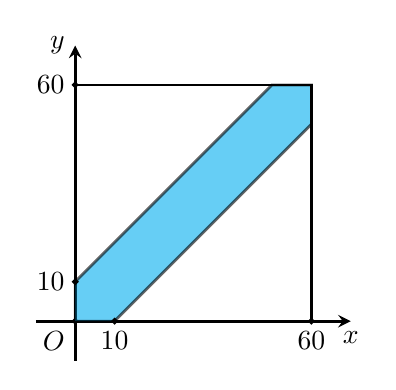
\begin{tikzpicture}[>=stealth, scale=0.5, line width=1pt]
				\draw[->] (-1,0) -- (7,0) node[below] {$x$};
				\draw[->] (0,-1) -- (0,7) node[left] {$y$};
				\draw[fill=black] (0,0) node[below left=-0.1] {$O$} circle (1.2pt);
				\draw[fill=cyan, opacity=0.6] (0,0) -- (0,1) -- (5,6) -- (6,6) -- (6,5) -- (1,0) -- (0,0);
				\draw (6,0)--(6,6)--(0,6);
				\draw[fill=black] (1,0) node[below] {$10$} circle (1.2pt);
				\draw[fill=black] (6,0) node[below] {$60$} circle (1.2pt);
				\draw[fill=black] (0,1) node[left] {$10$} circle (1.2pt);
				\draw[fill=black] (0,6) node[left] {$60$} circle (1.2pt);
			\end{tikzpicture}
		}
	}
\end{ex}
\Closesolutionfile{ans}
